% To je predloga za poročila o domačih nalogah pri predmetih, katerih
% nosilec je Blaž Zupan. Seveda lahko tudi dodaš kakšen nov, zanimiv
% in uporaben element, ki ga v tej predlogi (še) ni. Več o LaTeX-u izveš na
% spletu, na primer na http://tobi.oetiker.ch/lshort/lshort.pdf.
%
% To predlogo lahko spremeniš v PDF dokument s pomočjo programa
% pdflatex, ki je del standardne instalacije LaTeX programov.

\documentclass[a4paper,11pt]{article}
\usepackage{a4wide}
\usepackage{fullpage}
\usepackage[utf8x]{inputenc}
\usepackage[slovene]{babel}
\selectlanguage{slovene}
\usepackage[toc,page]{appendix}
\usepackage[pdftex]{graphicx} % za slike
\usepackage{setspace}
\usepackage{color}
\definecolor{light-gray}{gray}{0.95}
\usepackage{listings} % za vključevanje kode
\usepackage{hyperref}
\renewcommand{\baselinestretch}{1.2} % za boljšo berljivost večji razmak
\renewcommand{\appendixpagename}{Priloge}

\lstset{ % nastavitve za izpis kode, sem lahko tudi kaj dodaš/spremeniš
language=Python,
basicstyle=\footnotesize,
basicstyle=\ttfamily\footnotesize\setstretch{1},
backgroundcolor=\color{light-gray},
}

\title{Logistična regeresija}
\author{Tomaž Tomažič (63100281))}
\date{\today}

\begin{document}

\maketitle

\section{Uvod}

Cilj naloge je bil implementirati logistično regresijo in izgraditi model na določenih podatkih.
\section{Podatki}

Primer podatkov je v datotetki z 28 atributi in 60 primeri. Zadnji stolpec predstavlja skupino kateri posamezen primer pripada. Možni vrednosti sta le 0 in 1. Testiral sem tudi obsežnejše podatke z imenom GDS1059.

\section{Metode}

Nalogo sem rešil tako da sem uporabil priloženo ogrodje in ga smiselno dopolnil. Test sem pognal na različnih vrednostih lambda, da sem lahko raziskal vplivl regularizacije na napovedi. Zanimive stopnje regularizacije so mi bile pri lambda=0.0005 ~\ref{slika1}, lambda=0.05 ~\ref{slika2} in pri lambda=0.5~\ref{slika3}. Pri majhnem lambda je razvidno, da se prilagodimo podatkom v preveliki meri. Taka funkcija nam na prvi pogled izgleda optimalna, vendar ni nujno najbolj primerna za napovedovanje. Nekoliko boljše izgleda ~\ref{slika2} slika 2,  sej je tu dovoljeno manjše odstopanje. Preveč regularizirana funkcija pa je pri lambda=0.5 ~\ref{slika3}, saj niti ne ohranja intuitativne oblike.

\begin{figure}[htbp]
\begin{center}
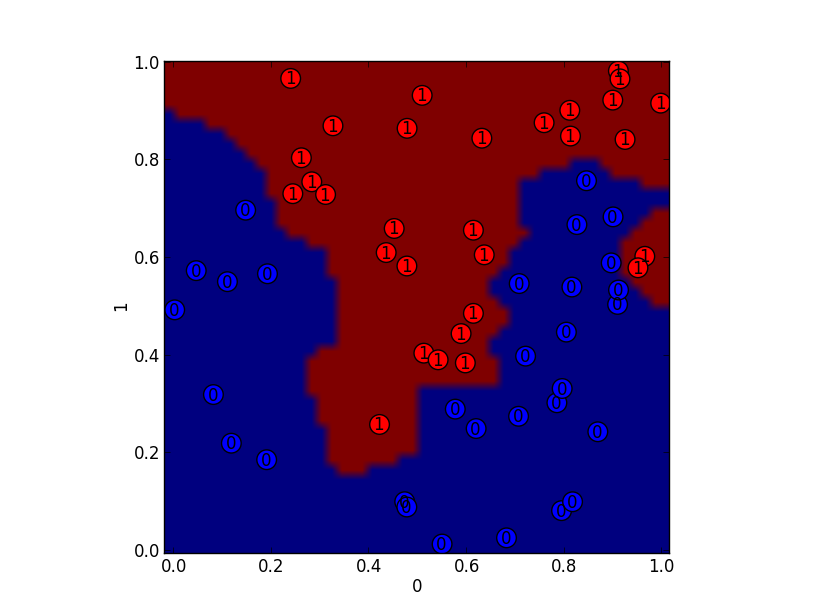
\includegraphics[scale=0.3]{fig1.png}
\caption{Izris podatkov v 2 dimenzijah pri določenem lambda}
\label{slika1}
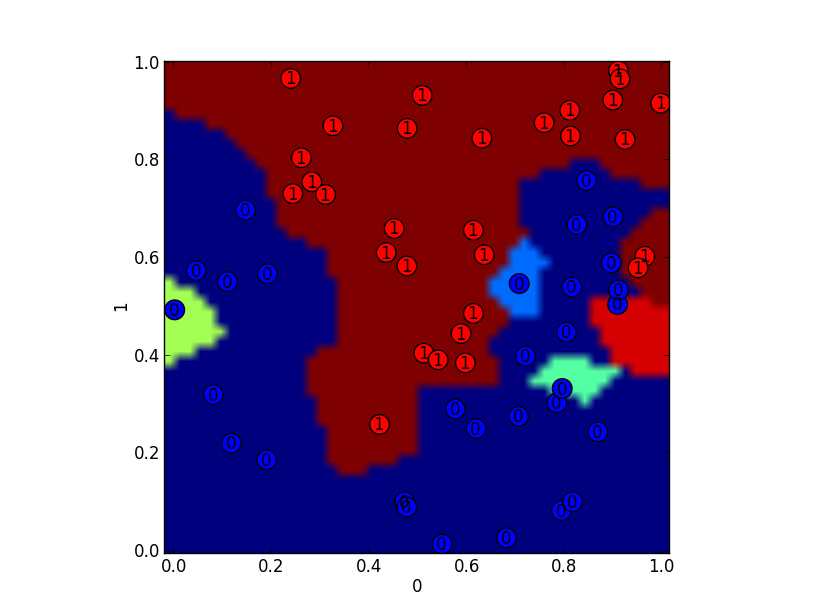
\includegraphics[scale=0.3]{fig3.png}
\caption{Izris podatkov v 2 dimenzijah pri določenem lambda}
\label{slika2}
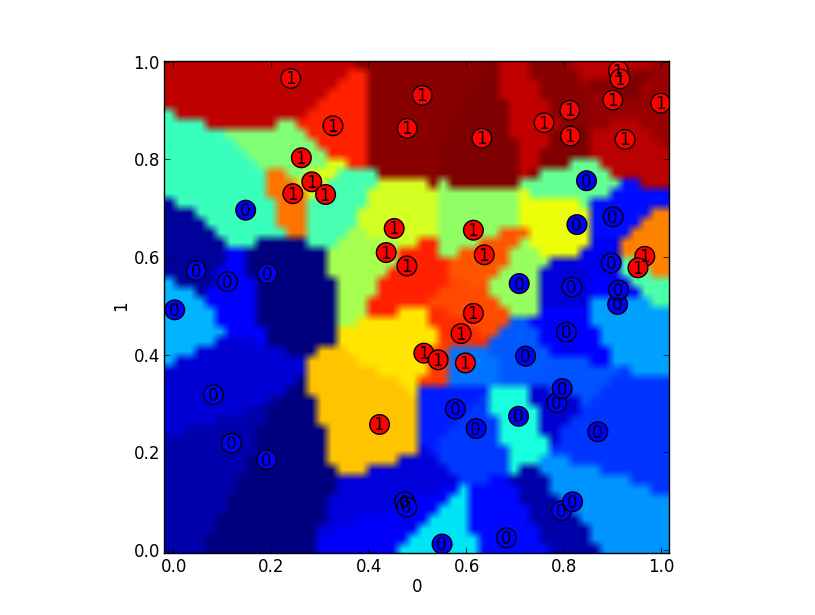
\includegraphics[scale=0.3]{fig2.png}
\caption{Izris podatkov v 2 dimenzijah pri določenem lambda}
\label{slika3}
\end{center}
\end{figure}




\section{Rezultati}


 S K-kratnim prečnim prevejranjem, sem testiral gradnjo modela in napovedovanje istih primerov, ki so v vhodnih podatkih. Preverjanje sem izvedel za različen nabor vrednosti lambda. Rezultati so prikazani v tabeli ~\ref{tab1}. Razvidno je, da točnost napovedovanja pri različnih lambdah niha. Nekje ima najvišjo vrednost, nato pa začne točnost  spet upadati.

\begin{table}[htbp]
\caption{K kratno preevrjanje točnosti.}
\label{tab1}
\begin{center}
\begin{tabular}{llp{3cm}}
\hline
točnost & vrednost lambda \\
\hline
0.74442447876 & 1e-05 \\
0.733398432863 & 5e-05 \\
0.783135711911 & 0.00025 \\
0.730327654345 & 0.00125 \\
0.734638081205 & 0.00625 \\
0.750608334012 & 0.03125 \\
0.727649151841 & 0.15625 \\
0.663830170228 & 0.78125 \\
\hline
\end{tabular}
\end{center}
\end{table}

Za  podatke GDS1059 sem dobil nalednje točnosti, ki so prikazane v tabeli ~\ref{tab2}. Stopnjo regularizacije ki bi bila najbolj primerna, nisem uspel najti, saj pri različnih lambda (0.0005~\ref{slika4}, 0.005~\ref{slika5}, 0.5~\ref{slika6}) dobim zelo podobne rezultate. Smiselno bi bilo opraviti permutacijski test in preveriti ali gre za naključne podatke.

\begin{table}[htbp]
\caption{K kratno preevrjanje točnosti v podatkih GDS1059.}
\label{tab2}
\begin{center}
\begin{tabular}{llp{3cm}}
\hline
točnost & vrednost lambda \\
\hline
0.768021461362 & 1e-05 \\
0.767515771074 & 5e-05 \\
0.767690926141 & 0.00025 \\
0.768451761935 & 0.00125 \\
0.759956150213 & 0.00625 \\
0.760401419028 & 0.03125 \\
0.741364988033 & 0.15625 \\
0.718926511778 & 0.78125 \\
\hline
\end{tabular}
\end{center}
\end{table}



\begin{figure}[htbp]
\begin{center}
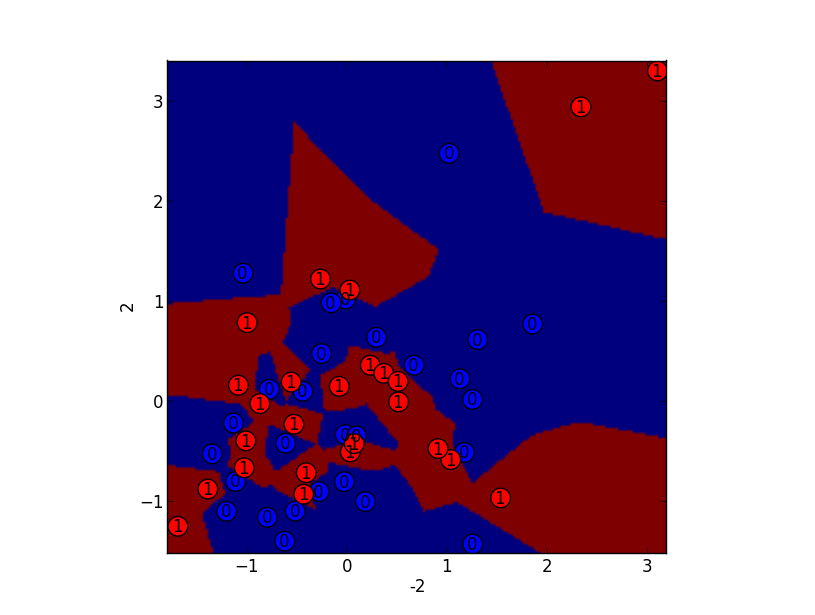
\includegraphics[scale=0.3]{fig11.png}
\caption{Izris podatkov v 2 dimenzijah pri določenem lambda}
\label{slika4}
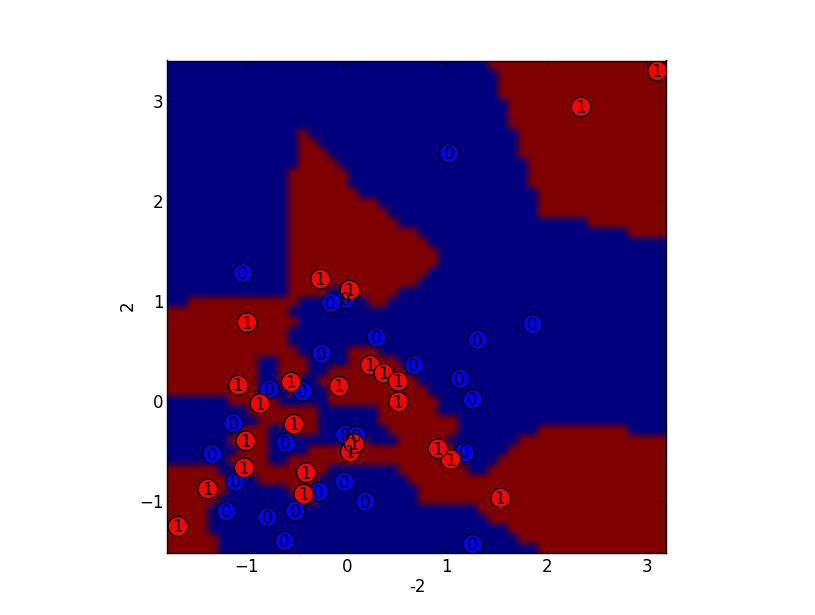
\includegraphics[scale=0.3]{fig12.png}
\caption{Izris podatkov v 2 dimenzijah pri določenem lambda}
\label{slika5}
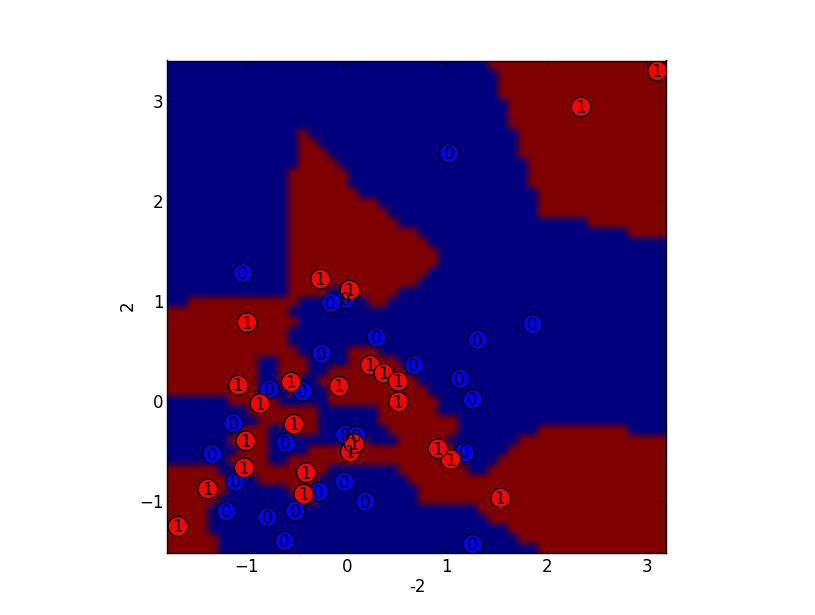
\includegraphics[scale=0.3]{fig13.png}
\caption{Izris podatkov v 2 dimenzijah pri določenem lambda}
\label{slika6}
\end{center}
\end{figure}
\section{Izjava o izdelavi domače naloge}
Domačo nalogo in pripadajoče programe sem izdelal sam.

\end{document}
